\documentclass{letter}
\usepackage{hyperref}
\usepackage{graphicx}
\usepackage{color}

\signature{Patrick Sanan}
\address{Dienerstrasse 15\\ Z\"{u}rich 8004\\ Switzerland}
\begin{document}
\begin{letter}{Stephanie Frequente\\CSCS Human Resources\\via Trevano 131\\6900 Lugano\\Switzerland}
\opening{Dear CSCS Scientific Computing Support Unit,}
I am writing to express my interest in the available position of Computational Scientist.

  I believe that I would be a valuable addition to the CSCS team as I have a very broad background in computational science, including a deep mathematical background, experience with software development, and experience with (geodynamics) application codes. I have a flexible and creative mindset, well-suited to quickly grasping problems from all areas of computational science. I enjoy the fast-paced, problem-solving nature of software development.

  I also have collaborative activities with the GFD group at ETH Zürich, and would look forward very much to continuing to work with them to develop, profile, accelerate, and hybridize their application codes. I have worked extensively with the \textsc{PETSc} library and its community.

  I already have familiarity with CSCS, its systems, and its staff, having been a postdoc on the GeoPC PASC project, working between USI Lugano and ETH Z\"{u}rich. I have taught at the CSCS Summer School for the last two years, have visited the center several times, and have run large jobs there. I've worked with Will Sawyer (a PI on our project) on a couple of occasions, including getting a CUDA-enabled build of PETSc running on Piz Daint. 

  I will be available after my current work contract expires, in Summer 2017. I am a native English speaker and a U.S./Irish dual citizen, with a B permit (under my Irish citizenship) from Canton Z\"{u}rich.
\closing{Sincerely,}
%\hfill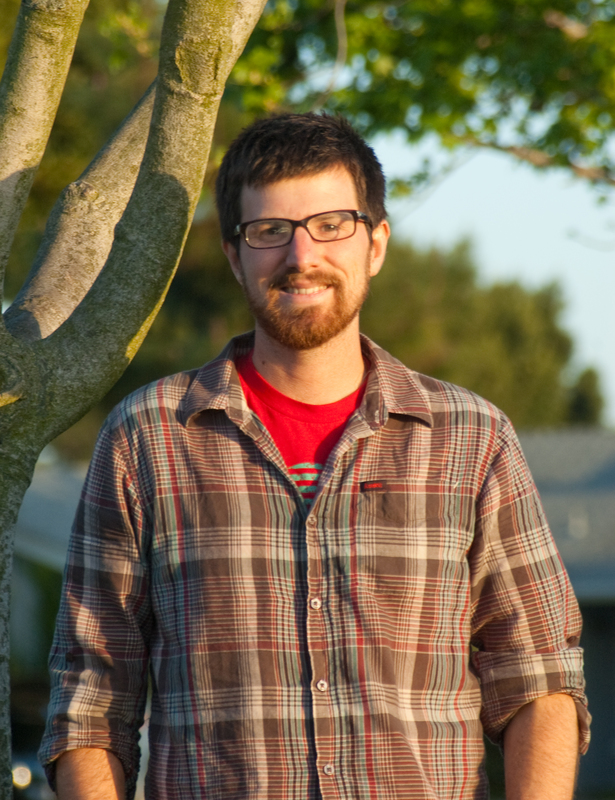
\includegraphics[width=170px]{sanan_patrick_portrait_small.jpg}
\end{letter}

\end{document}
